\section{Introduction}
Polymerase chain reaction (PCR) amplification during next-generation sequencing (NGS) library preparation can generate chimeric reads, which are artificial recombinant sequences formed when partially copied DNA fragments attach to different templates and are extended in later cycles \cite{Judo1998,Qiu2001}. Despite the high throughput and accuracy of Illumina sequencing, PCR-induced chimeras remain a persistent artifact that can affect downstream analyses and compromise genome assembly.

\begin{figure}[H]
    \centering
    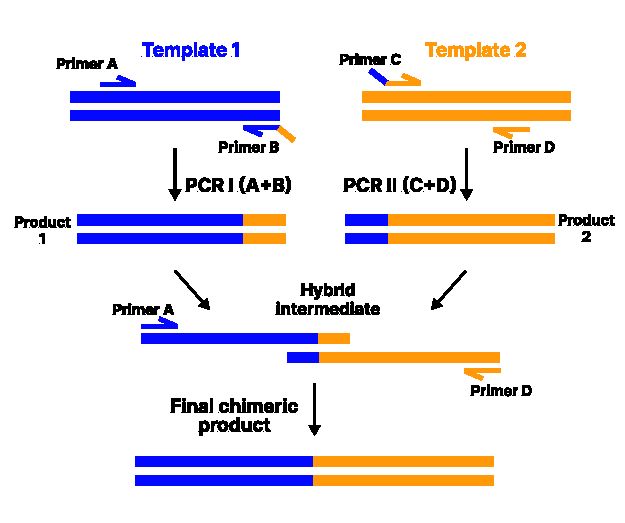
\includegraphics[width=0.78\textwidth]{figures/PCR_flat.pdf}
    \caption{Schematic illustration of PCR-induced chimera formation through incomplete extension and template switching, adapted from \cite{Sieber2011}.}
\label{fig:pcr_chimera}
\end{figure}

Mitochondrial genomes are particularly susceptible to this issue because they are small, circular, and often contain repetitive regions \cite{Boore1999,Cameron2014}. Under some conditions, junction-supporting artifacts may introduce misleading connections in assembly graphs, produce branching structures or fragmentation, or in some cases contribute to assembly failure \cite{Dierckxsens2017,Hahn2013,Jin2020}. Because many organelle assembly tools such as GetOrganelle \cite{Jin2020} and MITObim \cite{Hahn2013} assume that input reads are largely free of such artifacts, chimera-related assembly failure modes remain insufficiently addressed.

Many existing chimera detection approaches were originally developed for amplicon-based microbial community sequencing and often use differences in sequence frequency to help identify chimeras \cite{Edgar2011,Rognes2016}. These assumptions are not well aligned with single-species organellar sequencing, highlighting the need for a more specialized approach. A pipeline that detects chimeric reads from alignment and sequence irregularities can therefore be used as a pre-assembly filtering step.

This study introduces MitoChime, a pipeline for detecting PCR-induced chimeric reads in \textit{Sardinella lemuru} mitochondrial Illumina paired-end data. The pipeline extracts interpretable features from standard BAM and FASTQ artifacts, benchmarks supervised machine learning models together with a sequence-based convolutional neural network (CNN), and evaluates the effects of filtering on downstream assembly graph complexity.

\noindent\textbf{Contributions.} The study makes three main contributions. First, it develops a read-level feature set that combines alignment structure, clipping, k-mer discontinuity, and microhomology descriptors relevant to PCR-induced chimerism. Second, it benchmarks and tunes multiple classifiers while analyzing feature contributions to identify the most informative predictors. Third, it evaluates how filtering affects assembly graph complexity across different read depths and chimera rates to assess its benefits and limitations.

